\documentclass{fkssolpub}

\usepackage[czech]{babel}
\usepackage{fontspec}
\usepackage{fkssugar}
\usepackage{amsmath}
\usepackage{graphicx}

\author{Ondřej Sedláček}
\school{Gymnázium Oty Pavla} 
\series{74-I}
\problem{2} 

\begin{document}

\begin{figure}
	\begin{center}
		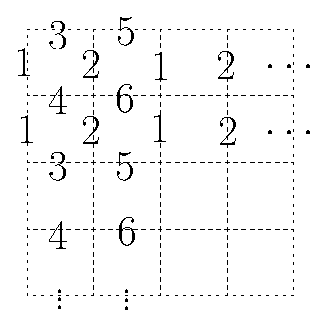
\includegraphics[width=0.5\textwidth]{2-fig}
	\end{center}
	\caption{Náčrtek toho, jakými stranami by mohly kostky sousedit}
	\label{fig:1}
\end{figure}

Z podmínky, že na bočních stěnách přilehlých kostek jsou stejná čísla, můžeme jednoduše odvodit, že v každém řádku nebo sloupci sousedí kostky právě dvěma bočními stěnami, které jsou protější. Tedy pokud bez újmy na obecnosti 1,2 jsou protější stěny, 3,4 jsou protější stěny a také 5, 6 jsou protější stěny, můžeme získat řádky a sloupce takové, kdy budou kostky sousedit stěnami 1 a 2, 3 a 4, nebo 5 a 6.

Teď bez újmy na obecnosti předpokládejme, že do krajního rohu jsme dali kostku tak, že vnikl řádek se stěnami 1,2 a sloupec se stěnami 3,4. Protože se čísla nemůžou na stěnách kostek opakovat, nemůže tedy už vzniknou nějaký řádek se stěnami 3,4 a nějaký sloupec se stěnami 1,2. Pokud tedy budeme už opakovat jen řádky se stěnami 1,2 a sloupce se stěnami 3,4, můžeme se na horních stěnách vyskytnout nejvýše 2 kostky. Když ale přidáme sloupec se stěnami 5,6, způsobíme tím, že nemůže existovat řádek se stěnami 5,6 a tedy kostky na každém řádku budou sousedit číslami 1,2, jelikož žádné další protější stěny šestistěnná kostka nemá. Z toho nutně plyne, že pak čísla 1,2 se nemůžou vyskytnout na horních stěnách kostek a největší počet různých čísel na horních stěnách kostek je 4.

Na obrázku výše pak je vidět takové rozmístění kostek, které dá právě řešení 4 (všechna ta čtyři čísla jsou v levém horním rohu). Tím je tedy důkaz u konce.

\end{document}
